%%%%%%%%%%%%%%%%%%%%%%%%%%%%%%%%%%%%%%%%%
% Short Sectioned Assignment
% LaTeX Template
% Version 1.0 (5/5/12)
%
% This template has been downloaded from:
% http://www.LaTeXTemplates.com
%
% Original author:
% Frits Wenneker (http://www.howtotex.com)
%
% License:
% CC BY-NC-SA 3.0 (http://creativecommons.org/licenses/by-nc-sa/3.0/)
%
%%%%%%%%%%%%%%%%%%%%%%%%%%%%%%%%%%%%%%%%%

%----------------------------------------------------------------------------------------
%	PACKAGES AND OTHER DOCUMENT CONFIGURATIONS
%----------------------------------------------------------------------------------------

\documentclass[paper=a4, fontsize=11pt]{scrartcl} % A4 paper and 11pt font size

\usepackage{graphicx}
\graphicspath{ {images/} }
\usepackage{verbatim}
\usepackage{textcomp}
\usepackage{changepage}
\usepackage[T1]{fontenc} % Use 8-bit encoding that has 256 glyphs
\usepackage{fourier} % Use the Adobe Utopia font for the document - comment this line to return to the LaTeX default
\usepackage[english]{babel} % English language/hyphenation
\usepackage{amsmath,amsfonts,amsthm} % Math packages

\usepackage{setspace}
\renewcommand{\baselinestretch}{1.3}
\usepackage{lipsum} % Used for inserting dummy 'Lorem ipsum' text into the template

\usepackage{color}

%\usepackage{biblatex}
%\addbibresource{sample.bib}

\usepackage{sectsty} % Allows customizing section commands
\allsectionsfont{\centering \normalfont\scshape} % Make all sections centered, the default font and small caps

\usepackage{fancyhdr} % Custom headers and footers
\pagestyle{fancyplain} % Makes all pages in the document conform to the custom headers and footers
\fancyhead{} % No page header - if you want one, create it in the same way as the footers below
\fancyfoot[L]{} % Empty left footer
\fancyfoot[C]{} % Empty center footer
\fancyfoot[R]{\thepage} % Page numbering for right footer
\renewcommand{\headrulewidth}{0pt} % Remove header underlines
\renewcommand{\footrulewidth}{0pt} % Remove footer underlines
\setlength{\headheight}{13.6pt} % Customize the height of the header

\numberwithin{equation}{section} % Number equations within sections (i.e. 1.1, 1.2, 2.1, 2.2 instead of 1, 2, 3, 4)
\numberwithin{figure}{section} % Number figures within sections (i.e. 1.1, 1.2, 2.1, 2.2 instead of 1, 2, 3, 4)
\numberwithin{table}{section} % Number tables within sections (i.e. 1.1, 1.2, 2.1, 2.2 instead of 1, 2, 3, 4)

\setlength\parindent{0pt} % Removes all indentation from paragraphs - comment this line for an assignment with lots of text

%----------------------------------------------------------------------------------------
%	TITLE SECTION
%----------------------------------------------------------------------------------------

\newcommand{\horrule}[1]{\rule{\linewidth}{#1}} % Create horizontal rule command with 1 argument of height

\title{	
\normalfont \normalsize 
\textsc{TRINITY COLLEGE DUBLIN, school of Mathematics} \\ [25pt] % Your university, school and/or department name(s)
\horrule{0.5pt} \\[0.4cm] % Thin top horizontal rule
\huge 5691 Seminar Report \# 2 \\ A Framework for an Automatic Hybrid MPI+OpenMP code generation \\ % The assignment title
\horrule{2pt} \\[0.5cm] % Thick bottom horizontal rule
}

\author{Gustavo Ramirez} % Your name

\date{\normalsize\today} % Today's date or a custom date

\begin{document}

\maketitle % Print the title

%----------------------------------------------------------------------------------------
%	PROBLEM 1
%----------------------------------------------------------------------------------------

\begin{comment}
\section{Problem description}

\begin{enumerate}
\item 
\item 
\item 
\item 
\end{enumerate}

\end{comment}

\newpage


\begin{comment}

USEFUL LINKS:

official sources for terminology:
-----
http://www.intel.com/content/www/us/en/support/topics/glossary.html
https://www-01.ibm.com/software/globalization/terminology/a.html
-----




about IMB processors:
-----

insert in google: list of ibm processors
https://en.wikipedia.org/wiki/List_of_IBM_products
https://www-01.ibm.com/software/passportadvantage/guide_to_identifying_processor_family.html
http://www.nextplatform.com/2015/08/10/ibm-roadmap-extends-power-chips-to-2020-and-beyond/
http://www.theverge.com/2015/7/9/8919091/ibm-7nm-transistor-processor
https://www.ibm.com/developerworks/ibmi/library/i-ibmi-7_2-and-ibm-power8/
-----




\end{comment}


%INTRO
\section{Introduction: BSP++ and the the framework built around it}

In a paper from Hamidouche \textit{et al.} \cite{hamidouche2}, the BSP++ library is developed. It basically consists in a tool for generating parallel code from a sequential version in an automated way.

The automatic creation of parallel code from a sequential one is, in general, a complicated and very interesting problem. Clearly, how difficult the implementation of the automatic translator will be depends on the initial assumptions, including the kind of problems that will be able to be automatically driven into a parallel version, and also the kind of hardware involved.

The framework discussed here was developed in an article by Hamidouche \textit{et al.} \cite{hamidouche}, and makes use of the BSP++ library; it is a system wrapping the BSP++ library, and adding the rest of layers necessary for making a completely automated system suitable for the creation of parallel code from its serial initial implementation.

There are multiple reasons for using such an automation tool. For instance, writing good parallel code requires both expertise and performance analysis, the latter being very time consuming, and the former implying a long time of hard work; even then, hybrid code can end up being inefficient due to many possible issues, like different types of overheads (at the MPI level, OpenMP level, etc.), load balancing, etc. Therefoce, one of the main motivations of such a tool is not dealing with all of that.

In short, the main goal of the framework described here is to produce efficient hybrid code for multi-core architectures from the source of a sequential function.



%The article presented \cite{hamidouche}



\section{Theory: BSP and SPMD}

\textbf{BSP} stands for Bulk Synchronous Parallel; it is synchronous in the sense that the work is divided in supersteps, and the estimations for execution times are then taken on each superstep. A diagram of one superstep in the BSP model can be seen in figure \ref{fig:bsp-description}.

\begin{figure}
\centering
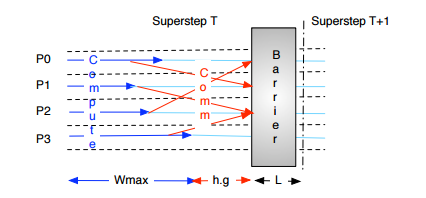
\includegraphics[width=1\linewidth]{bsp-description.png}
\caption{one superstep in the BSP model. Image taken from \cite{hamidouche}.} \label{fig:bsp-description}
\end{figure}

As seen from figure \ref{fig:bsp-description}, the BSP model consists of two overlaped stages, i.e. the computate stage and the communicate stage, the latter followed by a waiting stage, where basically calls to full synchronizations are made. A simple linear mathematical estimation of the execution time for such a superstep is of the form displayed in equation \ref{eq:time-superstep}, where:

\begin{itemize}
\item $\delta$: execution time for one superstep.
\item $W_{max}$: from the execution time for all the processes on their computations stage within one superstep, the maximum of all of those values.
\item $h$: maximal amount of data sent or received by one processor.
\item $g$: communication speed.
\item $L$: synchronization duration.
\end{itemize}

\begin{equation}
\delta = W_{max} + h\cdot g + L
\label{eq:time-superstep}
\end{equation}

The BSP model is subdivided in two submodels:

\begin{enumerate}
\item machine model: this model is composed of a set of processors linked through a communication medium supporting point-to-point communications and synchronizations. Some parameters associated to this submodel:
\begin{itemize}
\item $P$: number of processors.
\item $r$: speed, in FLOPS.
\item $g$: communication speed.
\item $L$: synchronization duration.
\end{itemize}
\item programming model: as displayed in figure \ref{fig:bsp-description}.
\end{enumerate}

Some cons of the BSP model:

\begin{itemize}
\item global synchronizations can cost a lot of execution time; this can become dominant for large parallel machines, where the number of communicating processors is too large. To reduce this problem, a possibility is launching threads within the processes, so that the amount of communications are reduced.
\end{itemize}

and some pros:

\begin{itemize}
\item it has a very simple analytical model, which implies a simple estimation of the execution time.
\item there is a performance improvement; the "best" number of processors and threads are found.
\end{itemize}

As mentioned in the last previous point, the "best" numbers of processors and threads are found. This basically implies an optimization on the execution time with some set of parameters, like communication speeds, finding then the best hybrid (MPI+OpenMP) configuration.

Going even further on the simplifications, a \textbf {SPMD} (Single Program Multiple Data) model is implied; this model implies that tasks are split up and run simultaneously on multiple processors with different input in order to obtain results faster. The SPMD assumption works very well when the OpenMP level is included, as each threads works on its own data and in a complete parallel way; SPMD implies, partly, not inserting serial sections between two parallel (OpenMP) sections. Using other mode different from SPMD might imply high thread creation overhead, and serial sections may become bottlenecks.

SPMD has several pros, such as the performance prediction becoming easier (there is a splitting into computation and communication times), false sharing is avoided, and load balancing is good, as all threads execute the same program.


\section{Implementation: analyzer, searcher and generator}

\subsection{Implementation specs}

The most significant assumptions over the system to be implemented are:

\begin{itemize}
\item it uses the BSP cost model to estimate execution time
\item the implementation finds the best configuration (number MPI processes and OpenMP threads)
\item generates hybrid code automatically
\end{itemize}

There are two inputs from the user: user source file containing sequential code and an XML describing some characteristics of the parallel code to be generated. The main output is hybrid MPI+OpenMP code.


\subsection{Analyzer}

This stage generates a numerical formula for execution time (with data size as parameter). It is used to estimate $T_{comm}$: it counts the number of cycles needed to execute a sequential function. The way it performs such a calculation, is with the use of the compiler Clang\footnote{see \cite{clang}.} (with all optimizations: -O3) to generate bytecode, which is then used as input for LLVM\footnote{see \cite{llvm}.} (which counts the number of cycles in the bytecode).

This is stage is further subdivided into:

\begin{itemize}
\item \textit{processor model} (no cache misses): the total execution time is calculated as $\sum_{i}C_{i}$ , with $C_{i}$ the hardware cost of each operation (e.g. load, store, etc.) $i$.
\item \textit{cache model} (for cache misses): total cost equals $\sum_{i}^{levels}(M_{i}{\cdot}PEN_{i})$, with the penalty $PEN_{i}$ given in nuber of cycles, and the number of cache misses $M_{i}$ is as given in equation \ref{eq:cache-misses-time}, where $j$ represents instructions, $\beta_{j}$ represents the amount of memory and $\gamma_{j}$ the number of references associated to that amount of memory for that instruction \# $j$.
\end{itemize}

\begin{equation}
\label{eq:cache-misses-time}
M_{i} = \frac{1}{CAPACITY_{i}}\sum_{j}(\gamma_{j}\beta_{j})
\end{equation}

Due to the simplicity of the BSP model, then the execution time for all levels (MPI, OpenMP, and more levels like CUDA is included) is as in equation \ref{eq:analyzer-exec-levels}.

\begin{equation}
\label{eq:analyzer-exec-levels}
T_{comm,k} = h_{k}\cdot g_{k}(P_{k}) + L_{k}(P_{k}), \ k \in \{ MPI, OpenMP \}
\end{equation}

At this point is when the \textit{system profile} comes in, which combines many benchmarks and sphinx\footnote{see \cite{sphinx}; sphinx is a tool for running performance tests of MPI, Pthreads and OpenMP.} to find $g_{k}(P_{k})$ and $L_{k}(P_{k})$.

Finally, the total execution time goes as a summation over all execution times, i.e. $T_{comm} = \sum_{k}T_{comm,k}$.


\subsection{Searcher}

This stage uses the previous formula and info from the \textit{system profile} to estimate cost for all possible configurations. The system profile retrieves execution time for basic operations, obtained either from the processor's manual and design specs, or by benchmarking.

It uses the XML and the data from the analyzer, in order to be able to find the best combination number of MPI processes and OpenMP threads.

Important factors taken into account by this stage are:

\begin{itemize}
\item number of MPI processes
\item number of threads per process
\item data size of the application
\end{itemize}

The searcher then plots a graph, as in figure \ref{fig:graph-searcher}. 

\begin{figure}
\centering
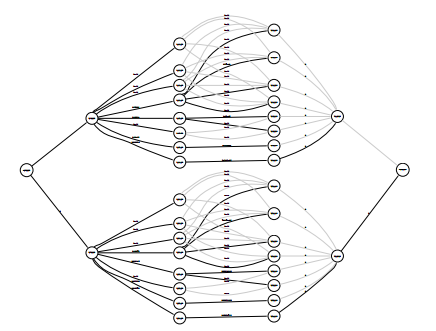
\includegraphics[width=0.8\linewidth]{searcher-graph.png}
\caption{graph created by the searcher stage before finding the best execution time. Image taken from \cite{hamidouche}.} \label{fig:graph-searcher}
\end{figure}

Each vertex is represented as $V(S_{i}, n, m, o)$, where $S_{i}$ represents the $i$-th superstep, $n$ the number of nodes, $m$ the number of processes and $o$ the number of threads, and an edge is a transition between two vertices, i.e. $V(S_{i}, n, m, o) \rightarrow V(S_{i+1}, n, m, o')$; the number of nodes and processes are fixed as MPI restrictions. After the graph is fully created, then Dijkstra's algorithm\footnote{see \cite{dijkstra}.} is used to find the shortest path, which implies shortest execution time.


\subsection{Generator: BSP++}

The third and final stage uses the configuration chosen through Dijkstra's algorithm and generates the corresponding hybrid code, with the use of the BSP++ library.

This part is based in a previous paper from the authors\footnote{see \cite{hamidouche2}.}. One of the most important points about the BSP++ library is that it implies a hybrid structure of the form displayed in figure \ref{fig:hybrid-structure}; as can be seen in figure \ref{fig:hybrid-structure}, the implementation is simply an insertion of OpenMP code in the computational MPI parts.

\begin{figure}
\centering
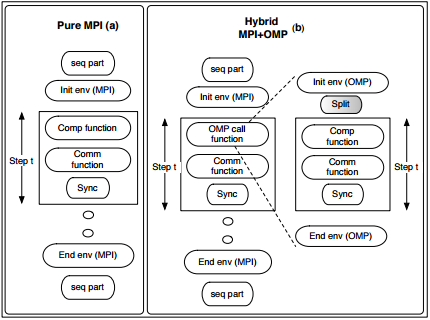
\includegraphics[width=0.8\linewidth]{generator-hybrid-struct.png}
\caption{hybrid structure on which the generator stage is based. Image taken from \cite{hamidouche}.} \label{fig:hybrid-structure}
\end{figure}


%CONCLUSIONS
\section{Benchmarks, results and conclusions}

\subsection{Benchmarks}

On testing the framework developed, four different benchmarks were used:
\begin{itemize}
\item inner product.
\item vector-matrix multiplication.
\item matrix-matrix multiplication.
\item parallel sorting by regular sampling algorithm.
\end{itemize}
Here, the first of those benchmarks is discussed; also, the hardware used consisted of 4 nodes, each node being a bi-processor with a bi-core and 2.6 GHz, 4 GB RAM and 2 MB of L2 cache.


\subsection{Results}

As can be seen from figure \ref{fig:results1}, for small data sizes the computation time is not larg enough, so that communication times represent a large portion of the total execution time when the number of processes is large (like in pure MPI); therefore, for small amounts of data, putting only threads to do all the computations is ideal, as the overhead of communicating between processes becomes important, and the double overhead of having MPI processes launching threads becomes important as well.

On the other hand, when the amount of data is large, as in figure \ref{fig:results2}, having as many cores as possible handling each of them one thread, is ideal; then, as seen in that figure, the fully hybrid version becomes the best option, as it leads to the lowest execution time.



\begin{figure}
\centering
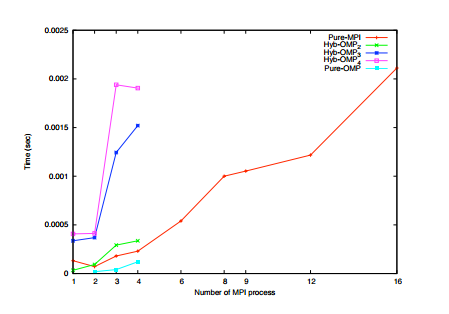
\includegraphics[width=0.8\linewidth]{results-plots1.png}
\caption{execution time for all possible configurations for the inner product program with a small data size (64 k). Image taken from \cite{hamidouche}.} \label{fig:results1}
\end{figure}


\begin{figure}
\centering
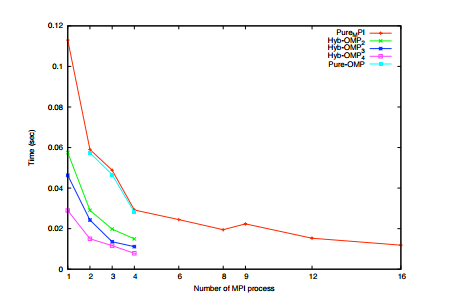
\includegraphics[width=0.8\linewidth]{results-plots2.png}
\caption{execution time for all possible configurations for the inner product program with a large data size (128 M). Image taken from \cite{hamidouche}.} \label{fig:results2}
\end{figure}



\subsection{Conclusions}

\begin{itemize}
\item The integration of more layers (e.g. CUDA) in the framework becomes relatively simple, as the assumptions imply BSP and SPMD.
\item The framework detects recursiveness automatically from the sequential code, and implements the parallel version taken this feature into account.
\item The described framework selects from pure MPI, pure OpenMP and hybrid MPI+OpenMP, and chooses the best hardware environment for the minimization of the total execution time.
\end{itemize}


%MATHEMATICAL DETAILS
%\section{Appendix}

%\subsection{Mathematical details of the Kernel Trick}


\newpage

%BIBLIOGRAPHY
%\section{References}

\begin{thebibliography}{1}

  \bibitem{hamidouche} Khaled Hamidouche, Joel Falcou, Daniel Etiemble {\em A Framework for an Automatic Hybrid MPI+OpenMP code generation.}  Proceedings of the 19th High Performance Computing Symposia (HPC '11) (2011)


  \bibitem{hamidouche2} Khaled Hamidouche, Joel Falcou, Daniel Etiemble {\em Hybrid bulk synchronous parallelism library for clustered smp architectures.}  Proceedings of the fourth international workshop on High-level parallel programming and applications (HLPP '10) (2010)

  \bibitem{clang} https://clang.llvm.org/


  \bibitem{llvm} http://llvm.org/

  
  \bibitem{sphinx} http://www.sphinx-doc.org/en/stable/

  \bibitem{dijkstra} http://www.personal.kent.edu/~rmuhamma/Algorithms/MyAlgorithms/GraphAlgor/ \\ dijkstraAlgor.htm



  %\bibitem{cancer_research} Costello \textit{et al.} {\em A community effort to assess and improve drug sensitivity prediction algorithms.} Nat Biotechnol. 2014 December; 32(12): 1202-1212.

  %\bibitem{impj}  The Japan Reader {\em Imperial Japan 1800-1945} 1973:
  %Random House, N.Y.

  %\bibitem{mehmet} Mehmet G{\"o}nen and Ethem Alpaydin. {\em Multiple Kernel Learning Algorithms} 2011: Journal of Machine Learning Research 12.

  %\bibitem{polly1} Polly Mitchell-Guthrie {\em Looking backwards, looking forwards: SAS, data mining, and machine learning} 2014: taken from: \\ http://blogs.sas.com/content/subconsciousmusings/2014/08/22/looking-backwards-looking-forwards-sas-data-mining-and-machine-learning/.

  %\bibitem{svm_linear} {\em Support Vector Machine Regression} Taken from:
  %http://kernelsvm.tripod.com/

  

  %\bibitem{fo} Bob Tadashi Wakabayashi {\em Anti-Foreignism and Western
  %Learning in Early-Modern Japan} 1986: Harvard University Press.

\end{thebibliography}




\end{document}